\documentclass[12pt]{scrartcl}

\usepackage[utf8]{inputenc}
\usepackage[naustrian]{babel}
\usepackage{caption}
\usepackage{graphicx}
\usepackage{verbatim}
\usepackage[T1]{fontenc}
\usepackage{lmodern}
\usepackage{subcaption}
\usepackage{amsmath}
\usepackage{amsfonts}
\usepackage{listings}
\usepackage{float}
\usepackage{tikz}
\usepackage{bookmark}
\usepackage{epigraph}

%pdfs
\usepackage{pdfpages}
\usepackage{tikz}

%page borders
\usepackage{geometry}
\geometry{left=2.5cm,right=2.5cm,top=3cm,bottom=2.5cm}

\usepackage{minted}
\setminted {
	%style=igor, %borland, autumn, vs
	encoding=utf-8,
	autogobble,
	tabsize=4,
	linenos,
	breaklines,
	%escapeinside=||
	%bgcolor=bg
	frame=single
}

\newenvironment{code}{\captionsetup{type=listing}}{}
\setlength\epigraphwidth{0.8\textwidth}

%title/footer/header values
\usepackage{titling}
\title{SWE Zusammenfassung}
\author{Elias Leonhardsberger}
\date{\today{}, Hagenberg}

%footer/header
%\usepackage[automark]{scrpage2}
%\pagestyle{headings}
%\clearscrheadfoot
%\ihead{\thetitle}
%\chead{\theauthor}
%\ohead{\today}
%\cfoot{Seite \pagemark}

\begin{document}
\maketitle
\tableofcontents

\pagebreak

\section{C++}
\subsection{Standard Library}
Der Namensraum \emph{std} ist für die Standardbibliothek von C++ und C reserviert.
Alle C Header-Dateien sind in C++ verfügbar, ihr Name ist immer mit einem \emph{c}
vorangestellt, z.B. \emph{cstdio} für \emph{stdio.h} in C.

\subsubsection{Strings}
Im gegensatz zu C, wo Strings als char-Arrays implementiert sind, gibt es in C++
die Klasse \emph{std::string}, die es ermöglicht mit Templates Strings aus \emph{char},
\emph{wchar\_t} oder einem beliebigen eigenen Typ zu erstellen. Die ersten beiden
Varianten sind bereits vordefiniert.

\begin{minted}{cpp}
typedef basic_string< char >   string;
typedef basic_string<wchar_t> wstring;
\end{minted}

\subsubsection{Ein-/Ausgabe}
In C und C++ gibt es keine in die Sprache eingebauten Ein-/Ausgabefunktionen. In C werden
die Funktionen aus \emph{stdio.h} verwendet, in C++ die Klassen aus \emph{iostream}.

Der Unterscheid ist, dass C++ mit Streams arbeitet, diese sind
\begin{itemize}
	\item typsicher
	\item implementierbar für eigene Klassen
	\item effizienter da man nicht auf interpretierte Formatzeichenketten angewiesen ist(z.B. \emph{\%d} für int)
	\item auf Zeichenebene Thread-sicher
\end{itemize}

\begin{figure}[H]
	\centering
	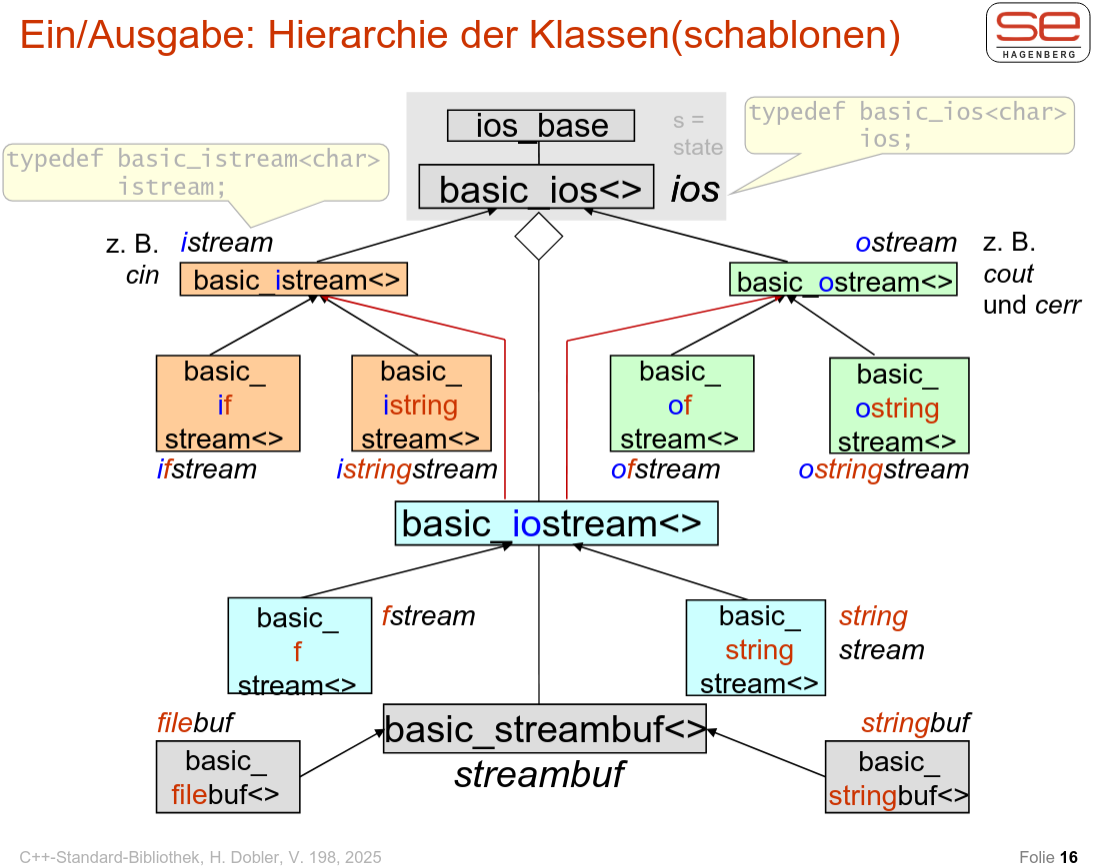
\includegraphics[width=0.49\textwidth]{images/cpp_1.png}
	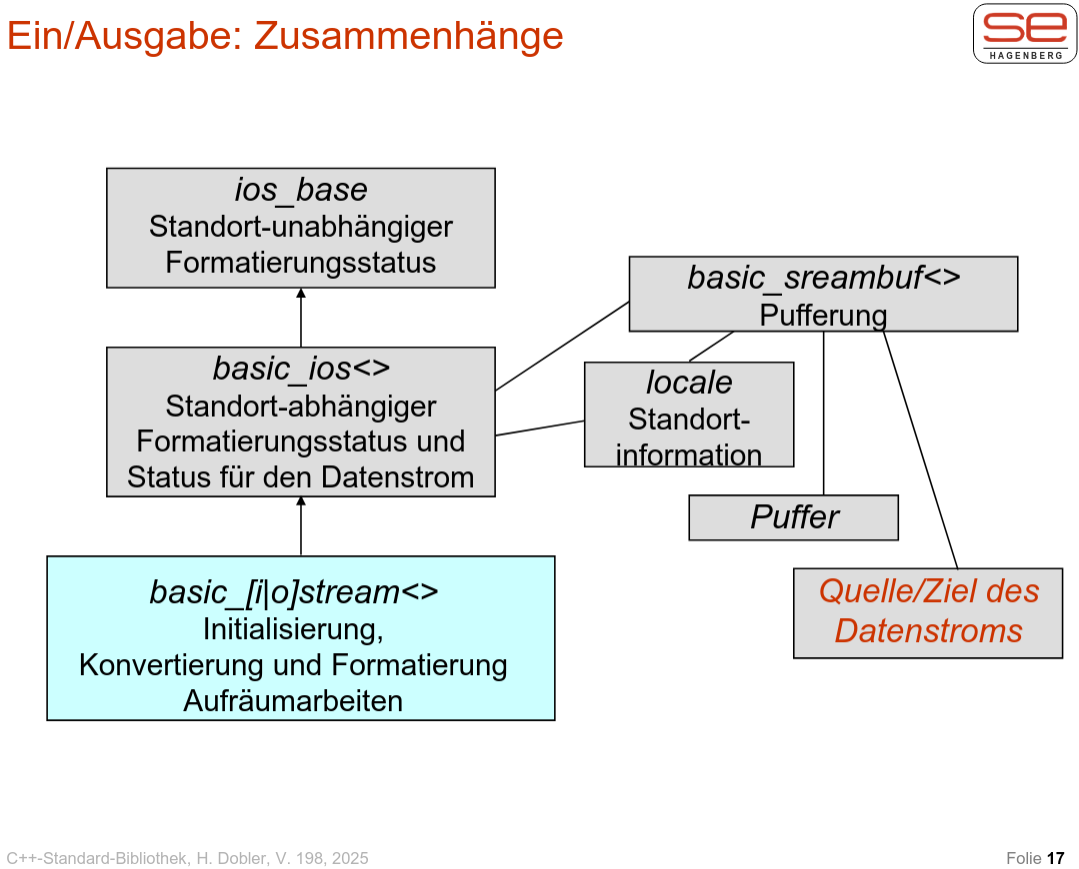
\includegraphics[width=0.49\textwidth]{images/cpp_2.png}
	\caption{Klassenhierarchie der Ein-/Ausgabeklassen in C++}
\end{figure}

Diese Streams sind in mehreren Header-Dateien aufgeteilt:
\begin{itemize}
	\item \textbf{iosfwd} für Vorwärtsdeklarationen(Sehr klein)
	\item \textbf{streambuf} für die Pufferung von Ein-/Ausgabe
	\item \textbf{istream} für die Eingabe
	\item \textbf{ostream} für die Ausgabe
	\item \textbf{iostream} für die Standard-Ein-/Ausgabe
	\item \textbf{fstream} für Dateiein-/ausgabe
	\item \textbf{sstream} für String-Ein-/Ausgabe
	\item \textbf{strstream} für für Char*-Ein-/Ausgabe
	\item \textbf{iomanip} für Ein-/Ausgabeformatierung
\end{itemize}

Flush kann auch mit Stream Aufrufen verkettet werden, z.B. \emph{cout << std::flush;}.
\emph{std::endl} flusht den Stream auch nachdem er einen Zeilenumbruch ausgegeben hat.
Achtung kann Performanceprobleme verursachen, da es den Puffer jedes Mal leert! Wenn mehrere
Zeilenumbrüche ausgegeben werden eher den folgenden Ausschnitt verwenden.

\begin{minted}{cpp}
stream << "\n"
\end{minted}

Es gibt auch diverse Manipulatoren, die das Verhalten von Streams beeinflussen.
\begin{itemize}
	\item \emph{std::dec} für Dezimalzahlen
	\item \emph{std::hex} für Hexadezimalzahlen
	\item \emph{std::oct} für Oktalzahlen
	\item \emph{std::setbase(n)} für die Basis der Zahlendarstellung
	\item \emph{std::setfill(c)} für das Füllzeichen
	\item \emph{std::setprecision(n)} für die Anzahl der Nachkommastellen
	\item \emph{std::setw(n)} für die Breite des Feldes
\end{itemize}
\pagebreak

\subsection{STL}
\epigraph{!!Diese Schablone hat keine Laufzeitprüfungen!!}{\textit{Doblers Foliensatz}}

Generische Programmierung statt OOP um den Code wiederverwendbar und effizient zu machen.

Die STL ist in mehrere Teile aufgeteilt:
\begin{itemize}
	\item \textbf{Behälter} für die Speicherung von Daten
	\item \textbf{Iteratoren} für den Zugriff auf die Daten
	\item \textbf{Algorithmen} für die Verarbeitung von Daten
	\item \textbf{Funktionsobjekte} für die Kapselung von Funktionen für andere Komponenten
	\item \textbf{Adapter} für die Anpassung von Behälter und Iteratoren
\end{itemize}

\begin{figure}[H]
	\centering
	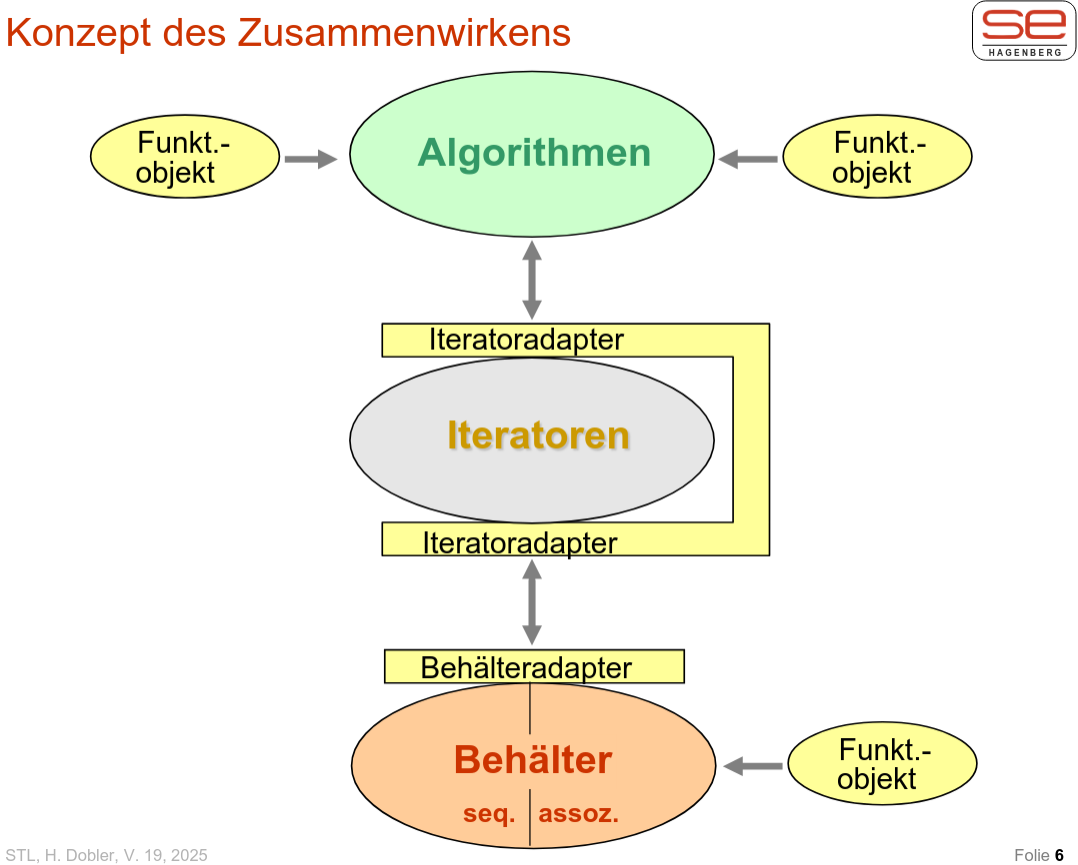
\includegraphics[width=0.8\textwidth]{images/stl_1.png}
	\caption{Verhältnisse der STL Komponenten}
\end{figure}

\subsubsection{Iteratoren}
Iteratoren sind eine Verallgemeinerung von Zeigern, die eine abstrakte Schnittstelle zwischen
Behältern und Algorithmen darstellen.

In der STL sind Iteratoren mithilfe von Ducktyping umgesetzt, das heißt, wenn die Schnittstelle erfüllt ist,
also die Methoden richtig implementiert sind, dann kann der Iterator verwendet werden.

\begin{figure}[H]
	\centering
	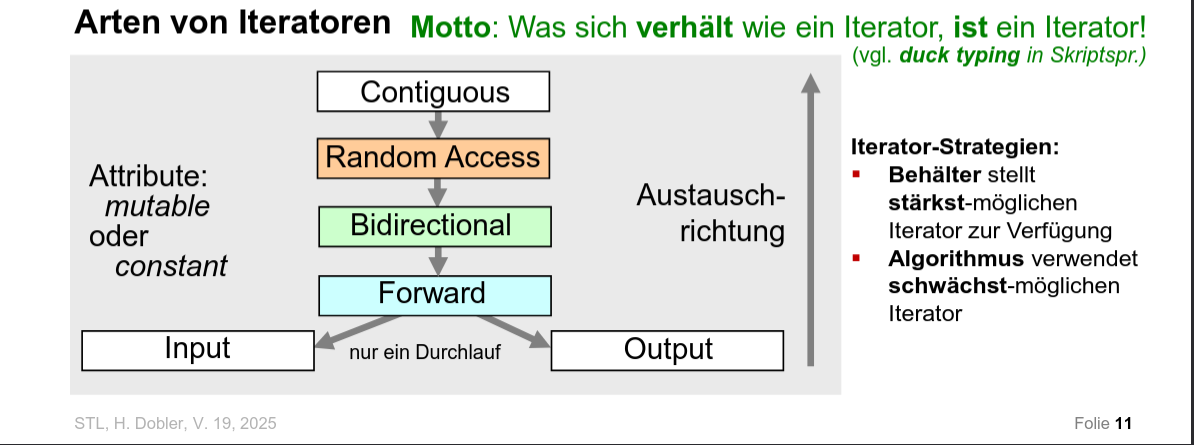
\includegraphics[width=0.8\textwidth]{images/stl_2.png}
	\caption{Iteratoren in der STL}
\end{figure}

Allgemein müssen Iteratoren die Vergleichsoperatoren \emph{==} und \emph{!=} implementieren, um zu überprüfen,
ob zwei Iteratoren auf das gleiche Element zeigen, und die Dereferenzierungsoperatoren \emph{*},
um auf das Element zuzugreifen.

Der \textbf{Vorwärtsiterator} implementiert zusätzlich den Inkrementoperator \emph{++}, um zum nächsten Element zu gelangen.

Der \textbf{bidirektionale Iterator} implementiert zusätzlich den Dekrementoperator \emph{--},
um zum vorherigen Element zu gelangen.

Der \textbf{Random-Access-Iterator} implementiert zusätzlich die Operatoren \emph{+}, \emph{-}, \emph{+=} und \emph{-=}, um auf ein
beliebiges Element im Behälter zuzugreifen, und die Vergleichsoperatoren \emph{<}, \emph{>}, \emph{<=} und \emph{>=},
um die Position der Iteratoren zu vergleichen. Dabei wird auch ein Differenztyp benötigt(z.B. \emph{ptrdiff\_t}).

Der \textbf{Input-Iterator} ist ein Vorwärtsiterator, der nur gelesen werden kann.

Der \textbf{Output-Iterator} ist ein Vorwärtsiterator, auf den nur geschrieben werden kann.
\linebreak

Streams und damit auch Dateien können mit dem \emph{istream\_iterator} und
\emph{ostream\_iterator} als Iteratoren verwendet werden.

Es gibt auch Adapter für Iteratoren, wie
\begin{itemize}
	\item \textbf{reverse\_iterator} für die Umkehrung der Iteration(v.rbegin() und v.rend())
	\item \textbf{back\_insert\_iterator} für das Einfügen von Elementen am Ende eines Behälters
	\item \textbf{front\_insert\_iterator} für das Einfügen von Elementen am Anfang eines Behälters
	\item \textbf{insert\_iterator} für das Einfügen von Elementen an einer bestimmten Position in einem Behälter
\end{itemize}

Die Einfügeiteratoren sind da um die Einfügeoperationen in Algorithmen zu abstrahieren.
\linebreak
Iteratoreigenschaften werden verwendet um verschiedene Implementierungen für verschiedene Iteratoren zu ermöglichen.
Die Eigenschaften sind. Außerdem wird der Wertetyp und er Distanztyp damit gespeichert.

\subsubsection{Behälter}
Behälter sind Klassen, die Daten speichern und verwalten. Es gibt verschiedene Arten von Behältern, die sich in ihrer
Implementierung und ihrem Verhalten unterscheiden. Die wichtigsten Behältertypen sind:

\begin{table}[H]
	\centering
	\begin{tabular}{ p{2.5cm} | p{7cm} | p{5cm} }
		Behältertyp            & Beschreibung
		                       & Verwendung                                                                        \\
		\hline
		\textbf{vector}        & Dynamisches Array, das hinten offen ist und schnellen direkten Zugriff ermöglicht
		                       & Standard für sequentielle Daten                                                   \\
		\hline
		\textbf{list}          & Doppelt verkettete Liste, die schnelle Einfüge-
		und Löschoperationen ermöglicht, aber keine schnelle Zugriffsfunktion
		                       & Wenn häufige Einfüg-/Löschungenoperationen erforderlich sind
		\\
		\hline
		\textbf{deque}         & beidseitig offenes dynamisches Array, das schnellen Zugriff
		auf beide Enden ermöglicht
		                       & Wenn häufige Einfüg-/Löschungenoperationen an beiden Enden erforderlich sind,
		aber direkter Zugriff auch wichtig ist                                                                     \\
		\hline
		\textbf{array}         & Schnittstelle für statisches Array
		                       & Wenn die Größe des Arrays zur Compilezeit bekannt ist und
		STL Algorithmen verwendet werden                                                                           \\
		\hline
		\textbf{forward\_list} & Minimale einfach verkettete Liste
		                       & Wenn Speicherverbrauch wichtig ist und nur Vorwärtsiteration benötigt wird        \\
	\end{tabular}
\end{table}

\begin{table}[H]
	\centering
	\begin{tabular}{ p{2.5cm} | p{7cm} | p{5cm} }
		Behältertyp               & Beschreibung
		                          & Verwendung                                                                \\
		\hline
		\textbf{stack}            & LIFO-Adapter für einen Behälter. Der genaue Behälter ist
		nicht spezifiziert, aber meist ein \emph{deque} oder \emph{vector}
		                          & Wenn nur die zuletzt hinzugefügten Elemente benötigt werden.              \\
		\hline
		\textbf{queue}            & FIFO-Adapter für einen Behälter. Der genaue Behälter ist
		nicht spezifiziert, aber meist ein \emph{deque} oder \emph{list}
		                          & Wenn nur die zuerst hinzugefügten Elemente benötigt werden.               \\
		\hline
		\textbf{priority\_ queue} & Adapter für einen Behälter, der die Elemente nach Priorität
		sortiert. Der genaue Behälter ist nicht spezifiziert, aber meist ein \emph{vector} oder
		\emph{deque}              & Wenn die Elemente nach Priorität sortiert werden müssen.                  \\
		\hline
		\textbf{set}              & Assoziativer Behälter, in dem die Elemente der Zugriffschlüssel
		sind.(Zugriff O(log n))
		                          & Wenn die Elemente als Zugriffschlüssel dienen.                            \\
		\hline
		\textbf{multiset}         & Set in dem Duplikate erlaubt sind
		                          & Wenn die Elemente als Zugriffschlüssel dienen aber Duplikate erlaubt sind \\
		\hline
		\textbf{map}              & Assoziativer Behälter, der zu jedem Schlüssel ein Element zuordnet.
		                          & Wenn auf die Elemente nach einem Schlüssel zugegriffen wird.              \\
		\hline
		\textbf{multimap}         & Map in der Schlüsselduplikate erlaubt sind
		                          & Wenn auf die Elemente nach einem Schlüssel zugegriffen wird,
		aber Duplikate erlaubt sind.                                                                          \\
	\end{tabular}
\end{table}

Assoziative Behälter sind entweder mit einem Rot-Schwarz-Baum oder einem Hash-Table implementiert.

\subsubsection{Funktionsobjekte}

Funktionsobjekte sind Objekte einer Klasse mit öffentlichem operator(). Sie können also wie Funktionspointer aufgerufen werden.
Da es sich aber um Objekte handelt, können sie auch Zustände speichern und so z.B. Zähler implementieren.

In den Folien wird auf 4 besondere Typen eingegangen:

\begin{figure}[H]
	\centering
	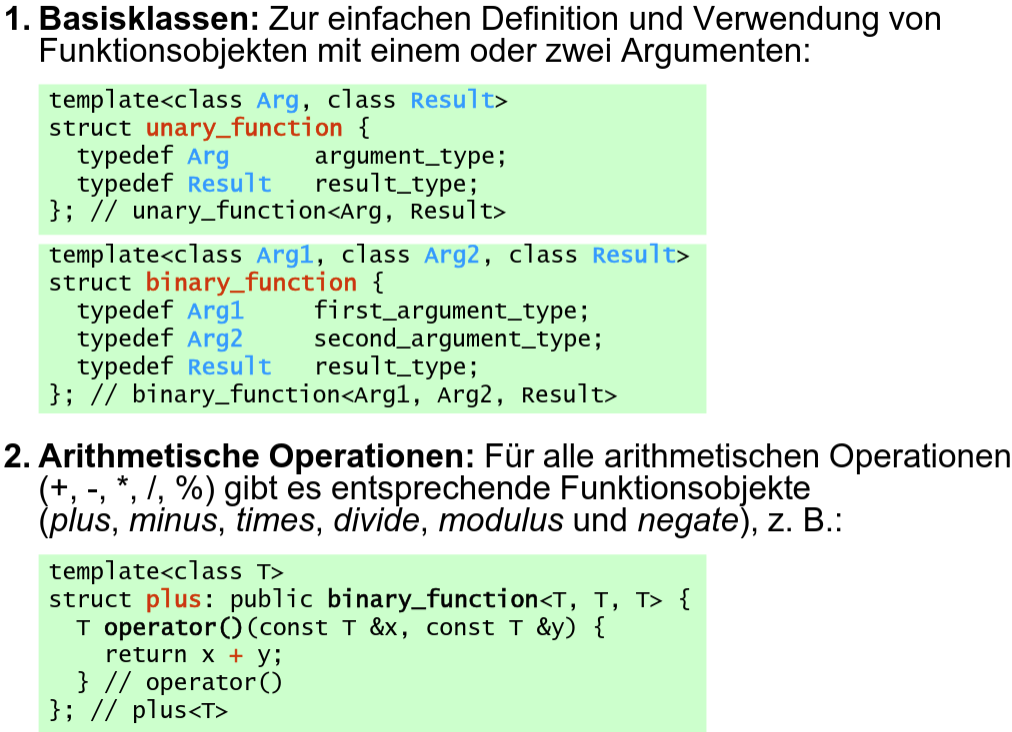
\includegraphics[width=0.49\textwidth]{images/stl_3.png}
	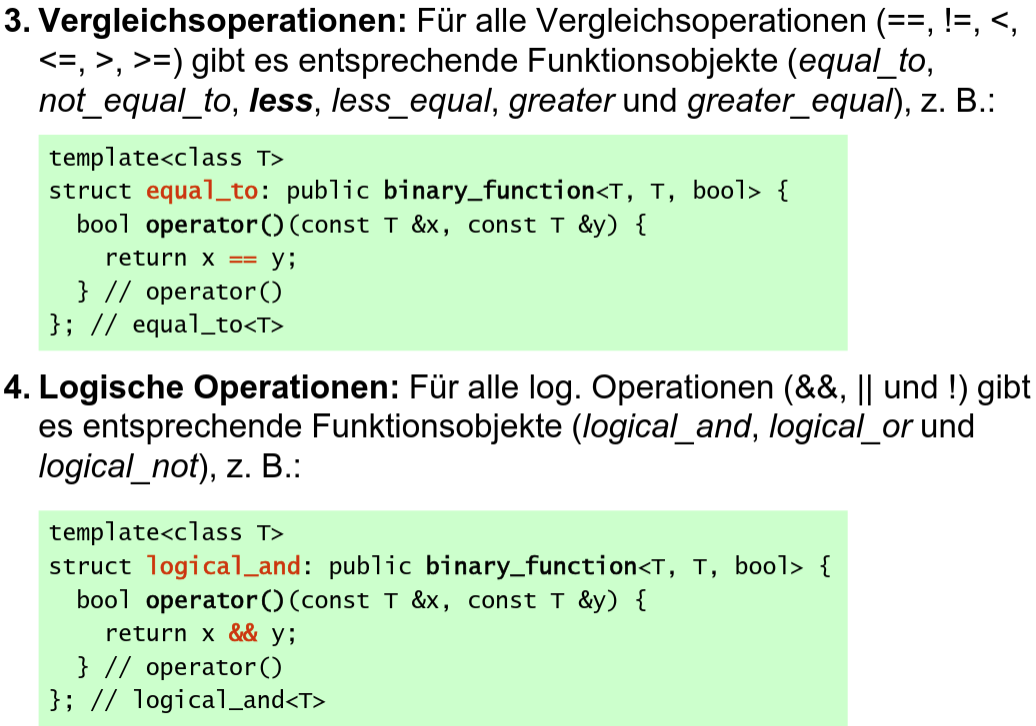
\includegraphics[width=0.49\textwidth]{images/stl_4.png}
	\caption{Funktionsobjekte in der STL}
\end{figure}

\subsubsection{Algorithmen}

Die Algorithmen in der STL sind durch Iteratoren unabhängig von den Behältern implementiert.
Parametrisiert werden sie mit Iteratortyp, Wertetyp oder Funktionsobjekten(z.B. Prädikat mit return Typ bool).
Davon können beliebig viele verwendet werden.

\begin{table}[H]
	\centering
	\begin{tabular}{ p{4cm} | p{11cm} }
		Algorithmus           & Beschreibung                                                                                                               \\
		\hline
		ohne Änderungen       &                                                                                                                            \\
		\hline
		\textbf{for\_each}    & Führt eine Funktion auf jedes Element eines Behälters aus                                                                  \\
		\textbf{find}         & Sucht ein Element in einem Behälter(mit ==)                                                                                \\
		\textbf{find\_if}     & Sucht ein Element in einem Behälter, das ein Prädikat erfüllt                                                              \\
		\textbf{count}        & Zählt die Anzahl der Vorkommen eines Elements in einem Behälter                                                            \\
		\textbf{count\_if}    & Zählt die Anzahl der Vorkommen eines Elements in einem Behälter, das ein Prädikat erfüllt                                  \\
		\textbf{equal}        & Vergleicht zwei Behälter auf Gleichheit(mit ==, Reihenfolge ist relevant)                                                  \\
		\textbf{mismatch}     & Vergleicht zwei Behälter auf Ungleichheit                                                                                  \\
		\hline
		mit Änderungen        &                                                                                                                            \\
		\hline
		\textbf{copy}         & Kopiert die Elemente eines Behälters in einen anderen Behälter                                                             \\
		\textbf{copy\_if}     & Kopiert die Elemente eines Behälters in einen anderen Behälter, die ein Prädikat erfüllen                                  \\
		\textbf{remove}       & Entfernt Elemente aus einem Behälter(mit ==)                                                                               \\
		\textbf{remove\_if}   & Entfernt Elemente aus einem Behälter, die ein Prädikat erfüllen                                                            \\
		\textbf{unique}       & Entfernt \textbf{aufeinanderfolgende} Duplikate aus einem Behälter                                                         \\
		\textbf{reverse}      & Kehrt die Reihenfolge der Elemente in einem Behälter um                                                                    \\
		\textbf{sort}         & Sortiert die Elemente eines Behälters in aufsteigender Reihenfolge                                                         \\
		\textbf{stable\_sort} & Sortiert die Elemente eines Behälters in aufsteigender Reihenfolge, aber behält die Reihenfolge von gleichen Elementen bei
	\end{tabular}
\end{table}
\pagebreak

\section{Java}

\subsection{Eigenschaften}

\begin{itemize}
	\item \textbf{Objektorientiert} - Objekt und Klassenbasiert mit Strukturierung in Paketen
	\item \textbf{Interpretierte Ausführung} - Java wird in Bytecode kompiliert, der von der Java Virtual Machine(JVM) interpretiert wird.
	\item \textbf{Architekturunabhängig} - Java-Programme können auf jeder Plattform, die eine JVM hat, ausgeführt werden.
	\item \textbf{Dynamisch und verteilt} - Klassen werden zur Laufzeit vom Interpreter geladen, es gibt keine statische Bindung.
	\item \textbf{Einfach} - Nur unbedingt notwendige Features. Zeiger, Mehrfachvererbung und Operatorüberladung sind nicht erlaubt.
	\item \textbf{Robust} - Starke Typisierung, keine Zeigerarithmetik, Laufzeitprüfungen bei Feldern, Ausnahmenbehandlung und automatische Speicherverwaltung.
	\item \textbf{Sicher} - Java nutzt Sandboxing, das den Zugriff auf Systemressourcen einschränkt.
	\item \textbf{Hohe Effizienz} - Nur 10 mal langsamer als C ;). Mit JIT-Compiler kommt oft ausgeführter Code näher an C.
	\item \textbf{Leichtgewichtige Prozesse} - Threads sind leichtgewichtig durch einfache Synchronisation und Kommunikation.
\end{itemize}

Ein Programm besteht aus beliebig vielen Klassen. Jede public Klasse muss in einer eigenen Datei liegen, die den gleichen Namen wie die Klasse hat.
Nur Klassen, Interfaces und Pakete haben globale Namen, es gibt keine globalen Variablen oder Funktionen.
Ein Paket ist eine Sammlung von logisch zusammengehörigen Klassen, die in einem Verzeichnis liegen. Die package-Deklaration muss am Anfang der Datei stehen.
Hierarchische Paketnamen werden 1 zu 1 auf Verzeichnisse abgebildet, z.B. \emph{java.lang} ist im Verzeichnis \emph{java/lang}.
Pakete der Java Standardbibliothek werden über die Property  \emph{java.home} gefunden,
Third-Party-Bibliotheken müssen über den Classpath angegeben werden.
\linebreak

Es gibt keinen Präprozessor, dadurch sind keine Makros, \#define oder \#include möglich.
Stattdessen gibt es die \emph{import}-Anweisung, die Klassen aus anderen Paketen importiert.
Für Konstanten gibt es \emph{static final} Membervariablen.

\subsection{Datentypen}

boolean ist kein Zahlenwert, also kann man nicht mehr damit rechnen. Es gibt keine unsigned Datentypen,
also sind alle Ganzzahligen Datentypen vorzeichenbehaftet.
\linebreak

Statt Pointer gibt es Referenzen, diese werden automatisch dereferenziert und man kann
nicht mit ihnen rechnen. Es gibt ein \emph{null}-Referenz Literal, die auf kein Objekt zeigt.

Objekte werden nicht bei der Definition statisch angelegt, sondern mit dem
\emph{new}-Operator dynamisch im Heap angelegt. Es gibt kein delete, da der Speicher
automatisch vom Garbage Collector freigegeben wird, wenn es keine Referenz auf ein Objekt mehr gibt.
\linebreak

Felder werden in Java mit mit eckigen Klammern angelegt. Es ist auch möglich, mehrdimensionale
Felder nicht rechteckig zu machen, also dass die Zeilen unterschiedlich lang sind.

\begin{figure}[H]
	\centering
	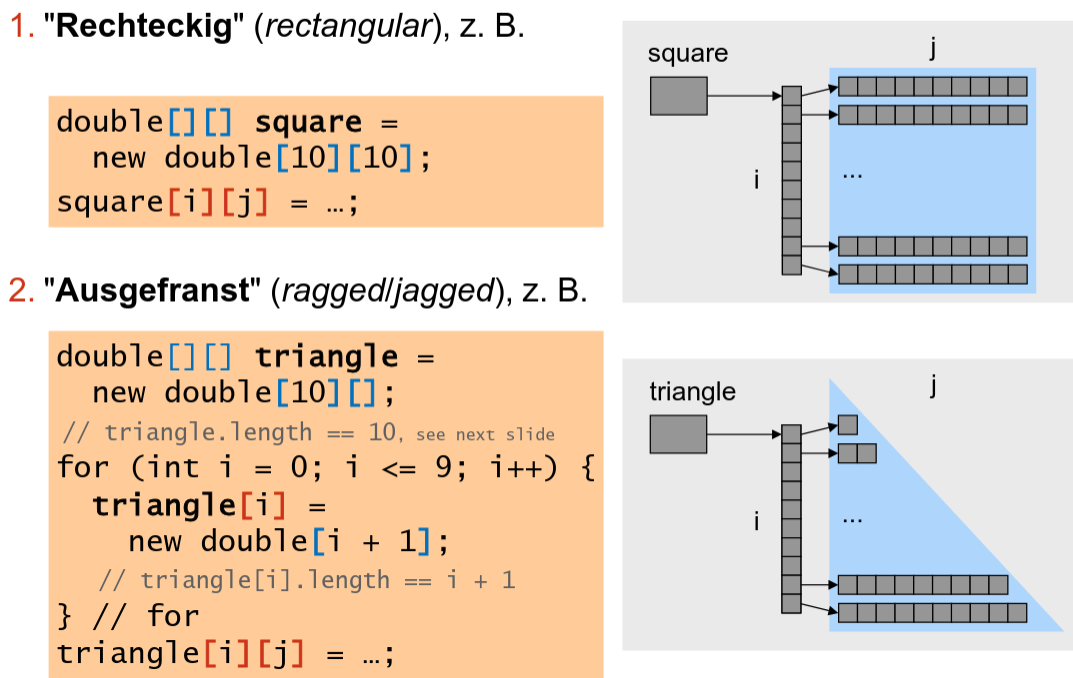
\includegraphics[width=0.8\textwidth]{images/java_1.png}
	\caption{Felder in Java}
\end{figure}

Strings sind Objekte der Klasse \emph{java.lang.String}, die immutable sind, also nicht verändert werden können.
Alle Stringoperationen erzeugen ein neues String-Objekt. Für Stringliterale werden automatisch
String-Objekte erzeugt.
Wenn man Strings bearbeiten möchte ohne neue Objekte zu erzeugen, muss man StringBuilder oder StringBuffer verwenden.

"Normale" Exceptions(Checked Exceptions) müssen entweder behandelt werden oder in der
Methodendeklaration mit \emph{throws} angegeben werden. Unchecked Exceptions sind RuntimeExceptions, die nicht behandelt werden müssen.
\pagebreak

\subsubsection{Klassen und Objekte}
\footnote{Ab hier wurde weniger Aufwand in die Zusammenfassung hineingesteckt. lol}
Initializer und Konstruktoren existieren.

\begin{figure}[H]
	\centering
	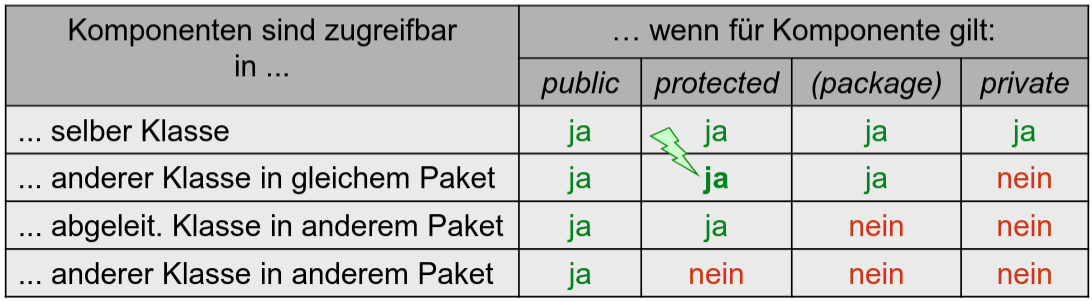
\includegraphics[width=0.8\textwidth]{images/java_2.png}
	\caption{Sichtbarkeiten in Java}
\end{figure}

Finalizer werden aufgerufen, wenn ein Objekt vom Garbage Collector freigegeben wird.
Sie sind nicht garantiert, dass sie aufgerufen werden, also sollten sie nicht für wichtige
Logik verwendet werden.\footnote{Schmutz}

Für Vererbung siehe Kapitel \ref{sec:syntaxvergleich}.

Mit Super kann auf die Basisklasse zugegriffen werden, wenn der Konstruktor der Basisklasse
aufgerufen werden soll, muss \emph{super()} im Konstruktor der abgeleiteten Klasse aufgerufen
werden.

Membervariablen können versteckt werden, indem man eine Variable mit dem gleichen Namen
in der abgeleiteten Klasse deklariert. Mit \emph{this} und \emph{super} kann auf die
jeweilige Variable zugegriffen werden.

Fürs Überschreiben von Methoden muss vor der Methode \emph{@Override} stehen.
Methoden mit dem Schlüsselwort \emph{final} können nicht mehr überschrieben werden.

\subsubsection{Interfaces und Abstrakte Klassen}

Klassen können als \emph{abstract} deklariert werden, wenn sie nicht instanziiert werden sollen.
Abstrakte Klassen können abstrakte Methoden enthalten, die in abgeleiteten Klassen implementiert werden
muss. Abstrakte Klassen können auch normale oder final Methoden enthalten.

Interfaces sind pur abstrakte Klassen, die nur abstrakte Methoden enthalten dürfen.

Mehrfachvererbung ist in Java von Klassen nicht erlaubt, aber eine Klasse kann
mehrere Interfaces implementieren.

\subsubsection{Generizität}

Bis Java 5.0 gab es in Java keine Generizität, also mussten alle Collections mit Polymorphismus
implementiert werden(nur Object Collections).

In Java werden Generics mit dem \emph{<>}-Operator
implementiert. Dabei wird der Typ in spitzen Klammern angegeben, z.B. \emph{List<String>}
für eine Liste von Strings. Anders als in C\# werden Generics in Java mit Type-Erasure implementiert,
das heißt, dass die Implementierung weiterhin mit Objekten arbeitet und die Typinformationen
nur zur Compilezeit geprüft werden können\footnote{Ebenso Schmutz}.


\subsubsection{Lamda-Ausdrücke und Streams}

Lamda-Ausdrücke wurden in Java 8 eingeführt und werden mit dem
\emph{->}-Operator geschrieben. Mit ihnen kann man anonyme Funktionen
erstellen, die zum Beispiel als Argumente an Methoden übergeben werden können.

Ein wichtiger Anwendungsfall sind Streams, die das Abarbeiten vom Elementen
in einer Collection vereinfachen. Man kann zum Beispiel mit einem Prädikat
und der \emph{filter}-Methode nur die Elemente einer Collection
auswählen, die das Prädikat erfüllen. Mit der \emph{map}-Methode kann man
jedes Element einer Collection durch eine Funktion transformieren.
Die \emph{reduce}-Methode kann verwendet werden, um eine Collection auf einen
einzigen Wert zu reduzieren, z.B. die Summe aller Elemente. \emph{forEach}
kann verwendet werden, um eine Funktion auf jedes Element einer Collection
anzuwenden, ohne eine Schleife zu verwenden.\footnote{Worse Linq}

\subsection{JCF}
\begin{table}[H]
	\centering
	\begin{tabular}{ p{4cm} | p{11cm} }
		Behältertyp         & Beschreibung                                                                                                                       \\
		\hline
		\hline
		\multicolumn{2}{c}{Vererbung von \emph{AbstactCollection}(Interface Collection) }                                                                        \\
		\hline
		\multicolumn{2}{c}{Vererbung von \emph{AbstractList}(Interface List)}                                                                                    \\
		\hline
		\textbf{ArrayList}  & Dynamisches Array, das hinten offen ist und schnellen direkten Zugriff ermöglicht                                                  \\
		\hline
		\textbf{Vector}     & Dynamisches Array, das hinten offen ist und schnellen direkten Zugriff ermöglicht, aber synchronisiert ist                         \\
		\hline
		\textbf{LinkedList} & Einfach verkettete Liste, die schnelle Einfüge- und Löschoperationen ermöglicht, aber keinen schnellen Zugriff auf Elemente bietet \\
		\hline
		\multicolumn{2}{c}{Vererbung von \emph{AbstractSet}(Interface Set)}                                                                                      \\
		\hline
		\textbf{HashSet}    & Implementierung einer Menge mit schneller Suche, Einfügen und Löschen                                                              \\
		\hline
		\textbf{TreeSet}    & Implementierung einer Menge, die Elemente in sortierter Reihenfolge speichert                                                      \\
		\hline
		\hline
		\multicolumn{2}{c}{Vererbung von \emph{AbstractMap}(Interface Map)}                                                                                      \\
		\hline
		\textbf{HashMap}    & Implementierung einer Map, die Schlüssel-Wert-Paare speichert und schnellen Zugriff auf die Werte ermöglicht                       \\
		\hline
		\textbf{TreeMap}    & Implementierung einer Map, die Schlüssel-Wert-Paare speichert und die Einträge in sortierter Reihenfolge hält                      \\
	\end{tabular}
\end{table}

\begin{table}[H]
	\centering
	\begin{tabular}{ p{4cm} | p{11cm} }
		Algorithmus                   & Beschreibung                                                                                                                             \\
		\hline
		\textbf{min} und \textbf{max} & Finden des minimalen oder maximalen Wertes in einer Collection, die Comparable implementiert oder ein Comparator angegeben ist           \\
		\hline
		\textbf{sort}                 & Sortiert die Elemente einer Collection in aufsteigender Reihenfolge, wenn Comparable implementiert ist oder ein Comparator angegeben ist \\
		\hline
		\textbf{binarySearch}         & Sucht ein Element in einer sortierten Collection, die Comparable implementiert oder ein Comparator angegeben ist                         \\
		\hline
		\textbf{reverse}              & Kehrt die Reihenfolge der Elemente in einer Collection um                                                                                \\
	\end{tabular}
\end{table}

\section{Softwaremuster}
\subsection{OOP}
\subsection{Gang of 4}
\subsection{MVC}
\subsection{Iterator}
\subsection{Composite}

\pagebreak
\section{Syntaxvergleich}\label{sec:syntaxvergleich}
Um den Syntax von C++ und Java zu vergleichen, hab ich ein kleines Beispielprogramm geschrieben mit:
\begin{itemize}
	\item einem Interface
	\item einer Basisklasse, die das Interface implementiert
	\item einer abgeleiteten Klasse, die von der Basisklasse erbt
	\item einer Iteratorimplementierung in der abgeleiteten Klasse
	\item einer Main-Methode, die ein Objekt der abgeleiteten Klasse verwendet
\end{itemize}

\subsection{C++}
\subsubsection{Interface}
\inputminted{cpp}{cpp/interface.h}
\subsubsection{Basisklasse}
\inputminted{cpp}{cpp/baseclass.h}
\subsubsection{Abgeleitete Klasse}
\inputminted{cpp}{cpp/derivedclass.h}
\subsubsection{Main}
\inputminted{cpp}{cpp/main.cpp}
\pagebreak

\subsection{Java}
\subsubsection{Interface}
\inputminted{java}{java/src/main/java/javademo/Interface.java}
\subsubsection{Basisklasse}
\inputminted{java}{java/src/main/java/javademo/Baseclass.java}
\subsubsection{Abgeleitete Klasse}
\inputminted{java}{java/src/main/java/javademo/Derivedclass.java}
\subsubsection{Main}
\inputminted{java}{java/src/main/java/javademo/Demo.java}
\pagebreak

\subsection{C\# kommt nicht zur Klausur - hab ich zu spät gesehen}
\subsubsection{Interface}
\inputminted{csharp}{csharp/IInterface.cs}
\subsubsection{Basisklasse}
\inputminted{csharp}{csharp/Baseclass.cs}
\subsubsection{Abgeleitete Klasse}
\inputminted{csharp}{csharp/Derivedclass.cs}
\subsubsection{Main}
\inputminted{csharp}{csharp/Program.cs}
\pagebreak

\end{document}